As already mentioned, we have used a structure of classes and methods similar to the one recommended in the assignments with some little modifications. Our model is based on the succession of layers within a Sequential container, which consist respectively of a Dense module and an activation function. We made the implementation choice to save the weights and biases inside the layer object, while gradients will be stored in the container. This is because during the backpropagation algorithm, which in our case takes place in the Sequential container, it is necessary to refer to all gradients in the network, while the subsequent weights update, performed by the optimizer, can be done separately. \\
The core of our framework is the Sequential module. When it is instantiated, the container receives as input all the Dense layers of the network. It add them in an ordered list and consequently initialize lists to store weight (dw) and bias (db) gradients.

\begin{minted}{Python}
def __init__(self, *args):
	super(Sequential, self).__init__()
	self.layers = [e for e in args if e.is_layer()]
	self.num_layers = len(self.layers)
	self.db = [FloatTensor(layer.bias.shape).zero_() for layer in self.layers]
	self.dw = [FloatTensor(layer.weigths.shape).zero_() for layer in self.layers]
	self.results = [] 
	self.activation = []
\end{minted}

Results and Activation lists will play an important role in the algorithm's evolution, as will be seen below. Result list will contain the outputs of the dense layers during the forward pass, while Activation will save the results of the corresponding activation functions. For an implementation issue the input layer during the backpropagation algorithm will be treated as a result of activation function, hence stored in the Activation list. Thinking about it, it is reasonable since it is what enter as input in the first layer of the net and it should be treated exactly the same as other input layers. 
\begin{figure}[H]
	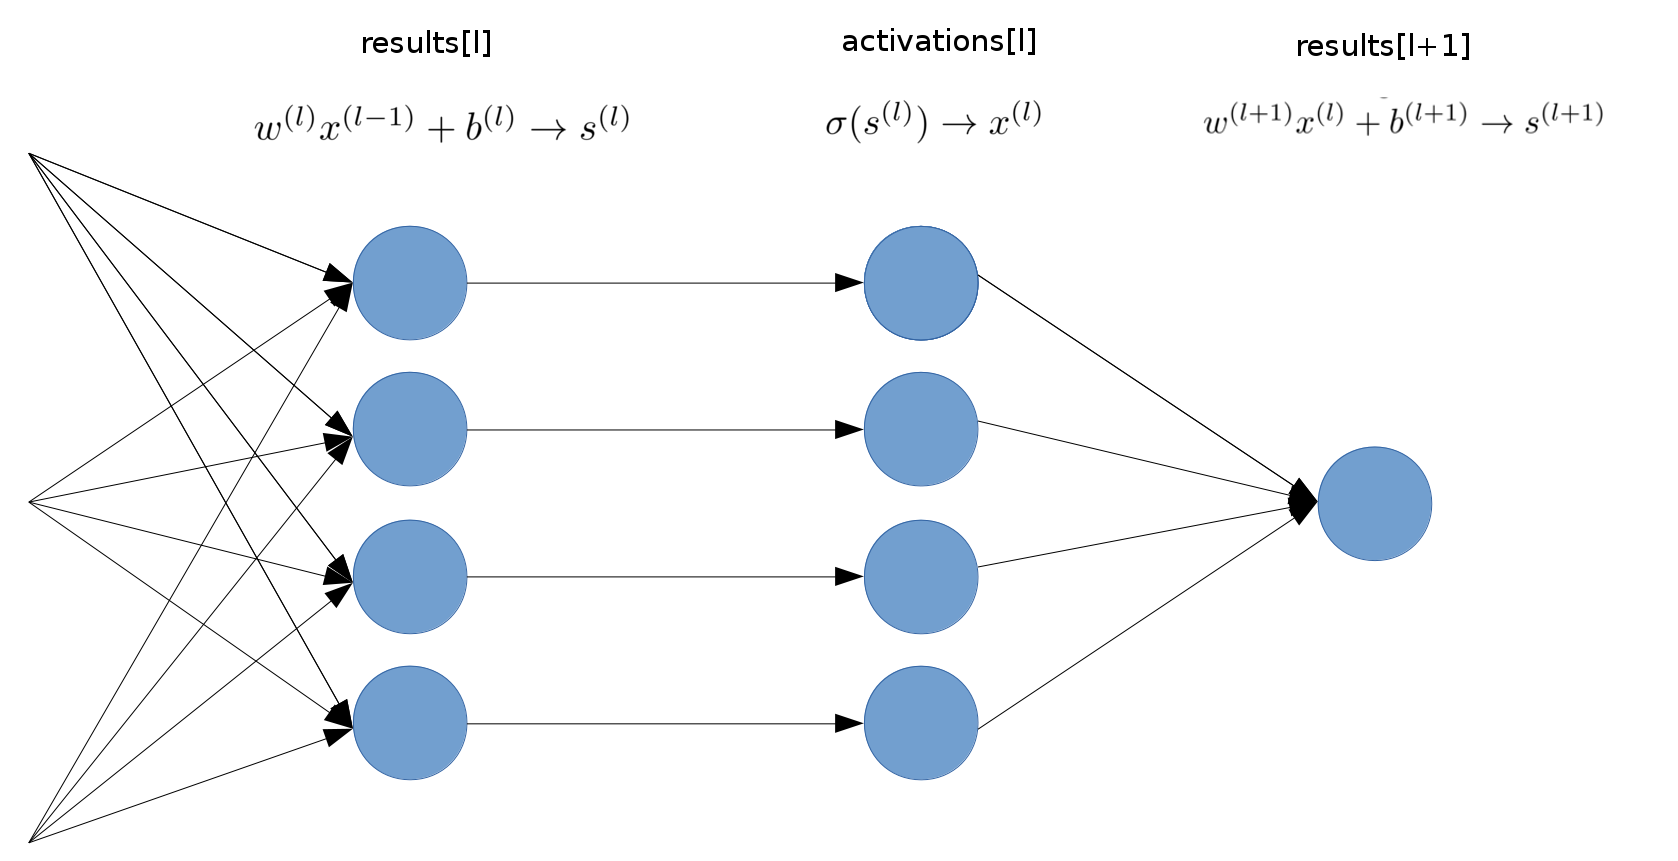
\includegraphics[width=0.8\textwidth]{Images/netowrk.png}
	\centering
\end{figure}
Thanks to the figure above our model structure can be easily understood. In fact we have separated the Dense layer that computes results from the activation layer that computes activations. 
\subsection{Backpropagation Algorithm Implementation}
\label{sect:Backpropagation}

\begin{minted}{Python}
def backward(self, loss, target, mini_batch):
    
    db = self.db
    dw = self.dw
    
    x_lt = self.activations[-1] 
    x_lb = self.activations[-2] 
    s_lt = self.results[-1]  
    dsigma = self.layers[-1].activation.backward(s_lt) 
    
    dldx = loss.prime(x_lt, target) 
    dlds = dsigma * dldx 
    
    db[-1].add_(dlds.sum(0)) 
    dw[-1].add_(x_lb.t().mm(dlds))
    
    for i in range(2, self.num_layers+1):
	    x_lt = self.activations[-i]
	    x_lb = self.activations[-(i + 1)]            
	    s_lt = self.results[-i]
	    
	    dsigma = self.layers[-i].activation.backward(s_lt)
	    w = self.layers[-i + 1].weigths
	    
	    dldx = (dlds).mm(w.t())
	    dlds = dldx * dsigma  
	    
	    db[-i].add_(dlds.sum(0))
	    dw[-i].add_(x_lb.t().mm(dlds)) 
    return dw, db
\end{minted}

During the algorithm implementation we decided to keep the computation of gradients of the output layer separate from those for the internal layers because they are slightly different. To fully understand and correctly implement the backpropagation algorithm we relied mainly on the slides provided by the course. 

\begin{figure}[H]
	\begin{minipage}{0.15\textwidth} 
		\begin{figure}[H]
			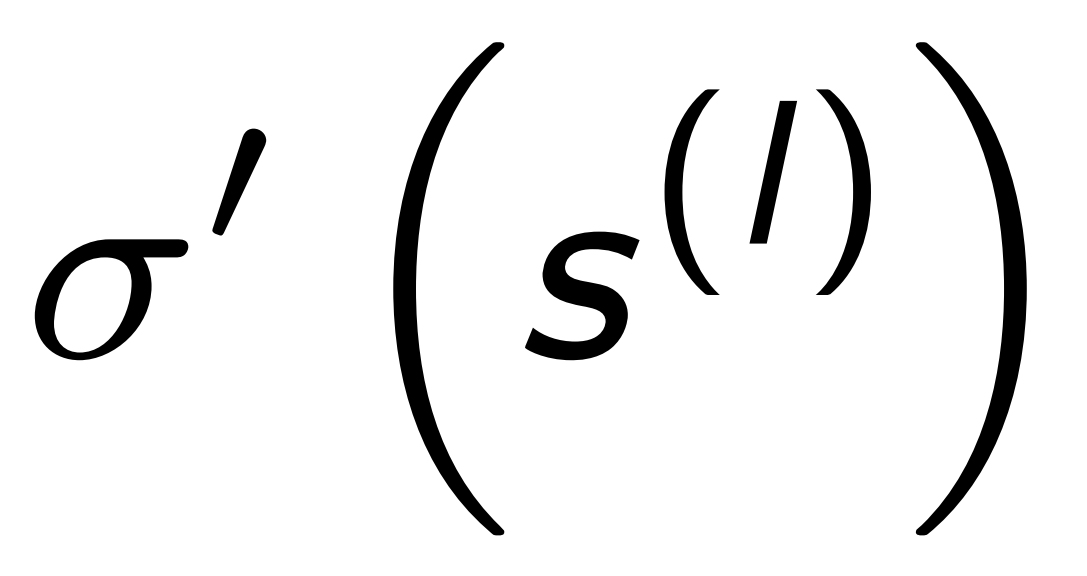
\includegraphics[width=0.5\textwidth]{Images/disgma.png}
			\centering
			\caption{dsigma}
			\centering
		\end{figure}
	\end{minipage} 
	\begin{minipage}{0.25\textwidth} 
		\begin{figure}[H]
			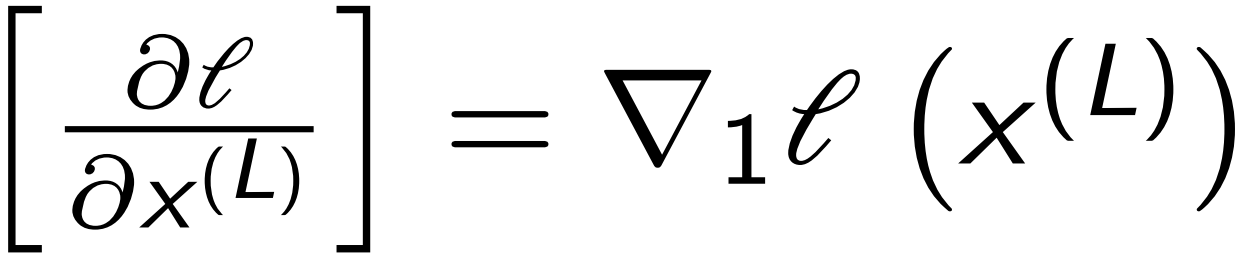
\includegraphics[width=0.9\textwidth]{Images/dldx_fin.png}
			\centering
			\caption{dldx output layer}
			\centering
		\end{figure}
	\end{minipage}
	\begin{minipage}{0.25\textwidth} 
		\begin{figure}[H]
			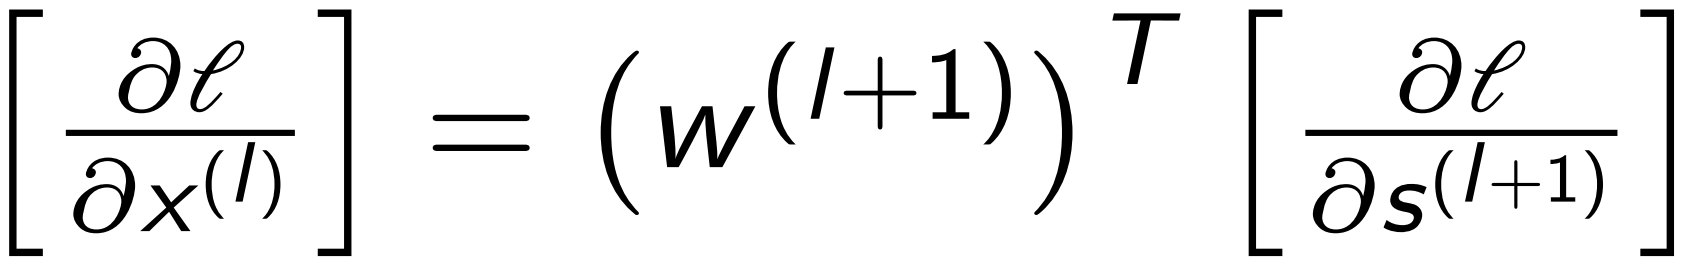
\includegraphics[width=0.9\textwidth]{Images/dldx_in.png}
			\centering
			\caption{dldx inner layer}
			\centering
		\end{figure}
	\end{minipage} 
	\begin{minipage}{0.25\textwidth} 
		\begin{figure}[H]
			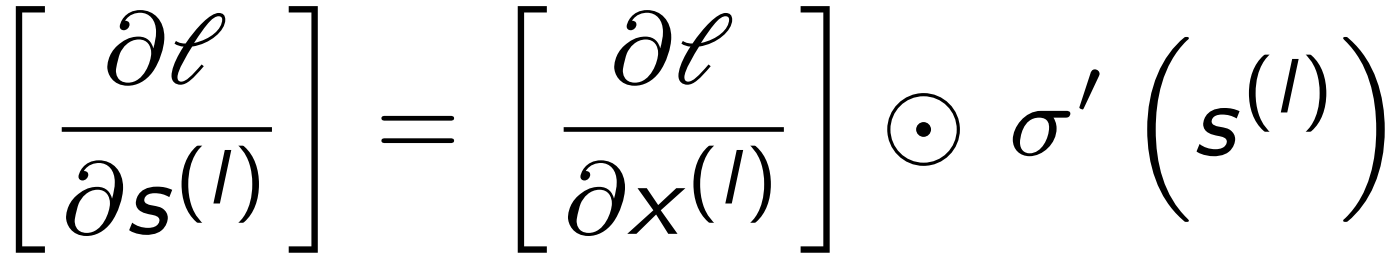
\includegraphics[width=0.9\textwidth]{Images/dlds.png}
			\centering
			\caption{dlds}
			\centering
		\end{figure}
	\end{minipage}
	\centering
\end{figure}

\begin{comment}
\begin{itemize}
	\item \textbf{disgma}: It contains the activation function derivative made with respect to the output of the previous dense layer.
	\item \textbf{dldx (output layer)}: It contains the derivative of the loss function, starting point of the algorithm. This step compares the final target and the network output to calculate the network output gradient.
	\item \textbf{dldx (inner layers)}: It is the derivative of the loss made with respect to the output of a specific layer. To calculate it, multiply the loss derivative obtained with respect to the output and the weights of the next layer. The algorithm, as you can see from the for loop that cycles in the opposite direction, starts from the network output and propagates back to the first input. For this reason when we are in an inner layer the derivatives made with respect to the next layer have already been calculated and therefore they can be used to propagate backwards the gradients. 
	\item \textbf{dlds}: It is the gradient of the output of the dense layer with respect to the final loss. It is calculated by multiplying the loss derivative of its own activation layer (the next one) and its derivative. This operation is the cause of vanishing gradient problem: if the network is too deep you risk that both factors become very close to zero, therefore dlds and all the gradients in previous layers would be stick to zero. This would lead to a dead net that doesn't change its weights and consequently stops learning.
\end{itemize}  

\end{comment}

The code has been properly commented in the source code; it can be useful to check also what support functions do, since they are not investigated in the report.

\subsection{Dense Layer}
\label{sect:Dense}
\begin{minted}{Python}
def __init__(self, in_neurons, out_neurons, activation):
    super(Dense, self).__init__()
    self.in_neurons = in_neurons
    self.out_neurons = out_neurons
    self.activation = activation
    self.weigths = FloatTensor(in_neurons, out_neurons).normal_() * 
	    math.sqrt(2.0 / in_neurons)
    self.bias = FloatTensor(out_neurons).zero_()
    self.error = 0
    
def forward(self, x):
    exceptions_check.checkFloatTensor(x)
    return x.mm(self.weigths).add(self.bias)
    
def backward(self, input):
    return input
\end{minted}
The definition of a Dense Layer is quite standard. We made the implementation choice to save the activation, taken as a parameter, in a specific field. For this reason the backward pass of this layer replicates only the input, while the derivative of the activation function will be executed during the backward pass calling activation.backward(input). \\
The initialization of the weights was problematic: at first the initialization was only done with a normal distribution, but we realized that with certain initial conditions the gradient lay down on a local minimum and blocked after a few epochs. At the end, after a detailed search on the web for weights initialization techniques, we found the solution should be multiplied by $\sqrt{\frac{2}{in\_neurons}}$. The problem was that the variance grows with the number of inputs, hence we have scaled it to make its variance $ \frac{1}{N} $, where N is the number of inputs.

\subsection{Optimizer}
\label{sect:Optimizer}

\begin{minted}{Python}
def step(self, model):
	 for i, layer in enumerate(model.layers):
		 layer.weigths -= self.lr * model.dw[i] 
		 layer.bias -= self.lr * model.db[i]
		 
def adjust_parameter(self, new_lr):
	 self.lr = new_lr
		 
\end{minted}
The step method is the core of the optimizer: since we have implemented only the SGD the updates on weights and biases are performed by subtracting the gradients multiplied by the learning rate, previously saved as the initial parameter of the optimizer. \\
We have given the possibility to update the learning rate during the training procedure. It can be very useful in more complicated problems when you want to decrease the learning rate after a specific number of epochs to increase precision and regularity.

\subsection{Loss}
\label{sect:Loss}

\begin{minted}{Python}
def apply(self, v, t):
	return (v - t.resize_(v.size())).pow(2).sum()

def prime(self, v, t):
	return 2 * (v - t.resize_(v.size()))  
\end{minted}
Apply and Prime are the two core methods of a Loss class. The former one computes loss instead the last one works on the derivative of the loss. \\
$ .resize(v.size()) $ must be inserted to handle specific 1D target tensors that can create dimensional problems.
   